\documentclass{standalone}
\usepackage[dvipsnames]{xcolor}
\usepackage{tikz}
\usetikzlibrary{arrows.meta, calc, positioning, shapes.geometric}

% General colors
\definecolor{MaRDI-blue}{RGB}{0,94,170}
\definecolor{MaRDI-orange}{RGB}{208,102,43}
\colorlet{MaRDI-grey}{black!40} % 40% black
\colorlet{MaRDI-gray}{MaRDI-grey}

% Light colors
\colorlet{MaRDI-light-blue}{MaRDI-blue!60}
\colorlet{MaRDI-blue-light}{MaRDI-light-blue}
\colorlet{MaRDI-lightest-blue}{MaRDI-blue!40}
\colorlet{MaRDI-blue-lightest}{MaRDI-lightest-blue}

\tikzset{%
  every path/.style={thick},
    edge/.style={%
        ->,
        >={Stealth[scale=1]},
    },
    usercode/.style={%
        rectangle,
        fill=MaRDI-orange,
        draw=black, thick,
        minimum width=3em,
        rounded corners=2pt,
        text=white,
        font=\footnotesize \sffamily,
        text centered,
    },
    lib/.style={%
        ellipse,
        fill=MaRDI-gray,
        minimum width=.12\linewidth,
        minimum height=.04\linewidth,
        rounded corners=2pt,
        text=white,
        font=\footnotesize \sffamily,
        text centered,
    },
    solver/.style={%
        rectangle,
        fill=MaRDI-blue,
        draw=black, thick, dashed,
        text=white,
        font=\footnotesize \sffamily,
        text centered,
        minimum width=3em,
        rounded corners=2pt,
    },
    grid/.style={%
      gray!20,
    }
}

\begin{document}
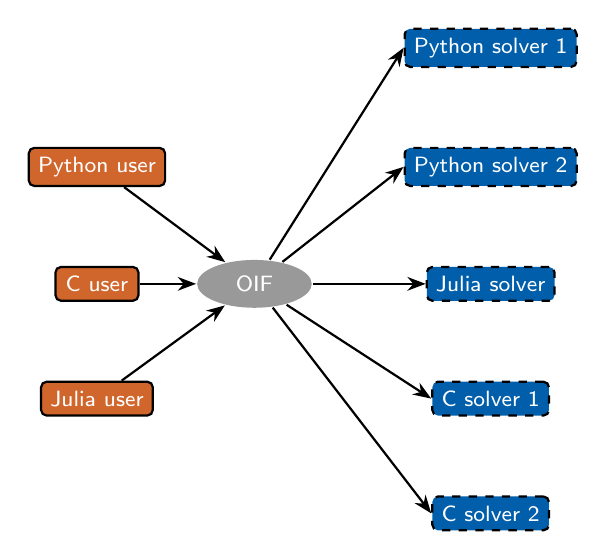
\begin{tikzpicture}
  % \draw[help lines] (-2, -2) grid (5, 5);
  \coordinate (left_side) at (-2, 0);
  \coordinate (right_side) at (3, 0);
  \coordinate (center) at (0, 0);

  \node [usercode] at (left_side) (user_c) {C user};
  \node [usercode, above=of user_c] (user_py) {Python user};
  \node [usercode, below=of user_c] (user_jl) {Julia user};

  \node [lib] at (center) (liboif) {OIF};

  \node [solver] at (right_side) (solver3) {Julia solver};
  \node [solver, above=of solver3] (solver2) {Python solver 2};
  \node [solver, above=of solver2] (solver1) {Python solver 1};
  \node [solver, below=of solver3] (solver4) {C solver 1};
  \node [solver, below=of solver4] (solver5) {C solver 2};

  \draw[edge] (user_py) -- (liboif);
  \draw[edge] (user_c) -- (liboif);
  \draw[edge] (user_jl) -- (liboif);

  \draw[edge] (liboif) -- (solver1.west);
  \draw[edge] (liboif) -- (solver2.west);
  \draw[edge] (liboif) -- (solver3.west);
  \draw[edge] (liboif) -- (solver4.west);
  \draw[edge] (liboif) -- (solver5.west);
\end{tikzpicture}
\end{document}